\section{Problem Formulation}
\label{sec:formulation}
In this paper, we would like to minimize the uplink energy consumption and model uploading time by exploiting the mobility of the {\IAVs}.
Because of their trade-off relation, the weighted summation of average uplink energy and uploading time (scheduling period duration) is used as the optimization objective.
Due to the randomness of {\IAVs}' trajectories, the joint scheduling design of the whole scheduling period, i.e., the transmission power and time allocation of all time slots, is a stochastic optimization problem, which can be formulated as a finite-horizon MDP.
We first define the system state, scheduling action, policy, and the cost function as follows.

\begin{definition}[State, Action and Policy]
    \label{def:mdp}
    In the $t$-th time slot, the local system state of the $m$-th {\IAV} is defined as
    \begin{align}
        \Stat_{m,t} &\define \Paren{ u_{m,t}, \vec{d}_{m,t} }, \forall m\in\carSet.
    \end{align}
    The global system state of the $t$-the time slot is defined as the aggregation of local system states of all {\IAVs}, thus
    \begin{align}
        \Stat_t &\define \Brace{ \Stat_{1,t}, \dots, \Stat_{M,t} }.
    \end{align}

    %<*tag:action>
    \revise{
        The scheduling action in the $t$-th time slot $\vec{A}_{t}$ consists of the allocation of transmission time and power of all {\IAVs}. Note that given the transmission time $\gamma_{m,t}$ and power $p_{m,t}$, the throughput of the $m$-th {\IAV} in the $t$-th time slot $r_{m,t}$ can be determined according to equation \eqref{eqn:vu}. Equivalently, the following definition of scheduling action is adopted for the elaboration convenience: 
        \begin{align}
            \vec{A}_{t} \define \Brace{ \gamma_{m,t}, r_{m,t} | \forall m\in\carSet }.
        \end{align}
    }%
    %</tag:action>
    A centralized scheduling policy in the $t$-th time slot $\Policy_{t}$ is a mapping from the global system state $\Stat_{t}$ to the scheduling action, thus,
    \begin{align}
        \Policy_{t}\paren{\Stat_t} &= \Paren{ \Policy^{\Gamma}_{t}(\Stat_t), \Policy^{R}_{t}(\Stat_t) },
    \end{align}
    where $\Policy^{\Gamma}_{t}: \Stat_{t} \to \set{\gamma_{m,t} | m\in\carSet}$ denotes the throughput allocation policy and $\Policy^{R}_{t}: \Stat_{t} \to \set{r_{m,t} | m\in\carSet}$ denotes the time allocation policy.
\end{definition}

Given the action of the $t$-th time slot, the state transition probability from the $t$-th time slot to the $(t+1)$-th one is given by
\begin{align}
    &\Pr\Bracket{ \Stat_{t+1} | \Stat_{t}, \vec{A}_{t} } =
    \nonumber\\
        &~~\prod_{m\in\carSet} \Pr\Bracket{ \vec{d}_{m,t+1} | \vec{d}_{m,t} }
        \cdot \indicator\Bracket{ u_{m,t+1}=u_{m,t}+r_{m,t} },
    \label{eqn:trans_prob}
\end{align}
where $\Pr\bracket{ \vec{d}_{m,t+1} | \vec{d}_{m,t} }$ denotes the transition probability of the $m$-th {\IAV}'s trajectory from the waypoint $\vec{d}_{m,t}  \in \tjSet_{m}$ to $\vec{d}_{m,t+1} \in \tjSet_{m}$.

The policy design aims to minimize a weighted sum of the average model uploading time of all {\IAVs} and the average transmission energy consumption.
To achieve this goal, we define the system cost of the $t$-th time slot ($\forall t$) as follows:
\begin{align}
    g_{t}\Paren{ \Stat_{t}, \mathbf{A}_t } =
        \indicator\Bracket{ \sum\limits_{m\in\carSet} u_{m,t} > 0} +
        \omega \sum_{m\in\carSet} { \gamma_{m,t} p_{m,t} },
    \label{eqn:func_g}
\end{align}
where the two items on the right-hand-side (RHS) count the costs of uploading time and energy consumption, respectively, and $\omega$ is the weight on the energy consumption.

Hence, the expected overall cost of the whole scheduling period can be written as
\begin{align*}
    \widebar{G}\Paren{ \Policy_1,\dots,\Policy_\T } \define \mathbb{E}_{ \Stat_1,\dots,\Stat_\T } \Bracket{ \sum_{t=1}^{\T} g_{t}\paren{ \Stat_t, \vec{A}_t } },
\end{align*}
where $\T$ denotes the maximum tolerable number of time slots in one scheduling period.
As a result, the scheduling problem can be written as
\begin{align}
    \textbf{P1: } &\min_{\Policy_1, \dots, \Policy_\T} \widebar{G}\Paren{ {\Policy_1,\dots,\Policy_\T} }
    \label{eqn:p1_eqn}
    \\
    &\text{s.t.~~~~}
    \gamma_{m,t} \geq 0, \forall t, m\in\carSet
    \label{eqn:p1_cons_second}
    \\
    &~~~~~~\sum_{m\in\carSet} \gamma_{m,t} \leq 1, \forall t
    \label{eqn:p1_cons_last}
    \\
    &~~~~\sum_{ t=T_{\text{comp},m}+1 }^{\T} r_{m,t} \geq U, \forall m\in\carSet
    \\
    &~~~~p_{m,t} \leq P_{\max}, \forall t, m\in\carSet.
    \label{eqn:p1_cons_first}
\end{align}

In order to solve the above finite-horizon MDP, we first introduce the following Bellman's equations:
\begin{align}
    V_{t}(\Stat_t) =& \min_{\Policy_{t}(\Stat_t)} \Brace{ g_{t}\Paren{ \Stat_t, \vec{A}_t } +
    \nonumber\\
    &\sum_{\Stat_{t+1}} \Pr\Bracket{ \Stat_{t+1} | \Stat_{t}, \vec{A}_t } \cdot V_{t+1}(\Stat_{t+1})
    }, t=1,\dots,T,
    \label{eqn:p1_blm}
\end{align}
where the value function of the optimal policies in the $t$-th time slot is given by
\begin{align}
    V_{t}(\Stat_{t}) \define \min_{\Policy_{t},\dots,\Policy_{\T}}& \mathbb{E}_{\Stat_{t},\dots,\Stat_{\T}}
    \Bracket{
        \sum_{\tau=t}^{\T} g_{\tau}\paren{ \Stat_{\tau}, \vec{A}_{\tau} } | \Stat_{t}
    }.
    \label{eqn:p1_val}
\end{align}

As a remark notice that in finite-horizon MDP, the value functions are usually heterogeneous for different time slots. The optimal time and throughput allocation policies can be obtained by solving the RHS of equation \eqref{eqn:p1_blm}.
However, the problem {\bf P1} is difficult to solve.
On one hand, the transition probability of {\IAVs}' trajectories in equation (\ref{eqn:trans_prob}) for a particular road network can hardly be obtained, unless extensive real experiments can be conducted on the road network beforehand.
On the other hand, the optimal value functions depend on the global system state, which grows exponentially with respect to the number of {\IAVs}.
Therefore, it is infeasible to calculate the value functions for each global system state before the online scheduling.

In order to address the above issues, a decentralized solution framework driven by a high-fidelity traffic simulation platform, namely {\fwName}, is proposed in this paper.
Particularly, the {\fwName} simulator is first proposed in Section \ref{sec:framework} to obtain the waypoint transition probabilities.
Then the {\fwName} optimizer is proposed in Section \ref{sec:new_framework} to address the issue of computational complexity in a decentralized manner.

\begin{figure*}[htp!]
    \centering
    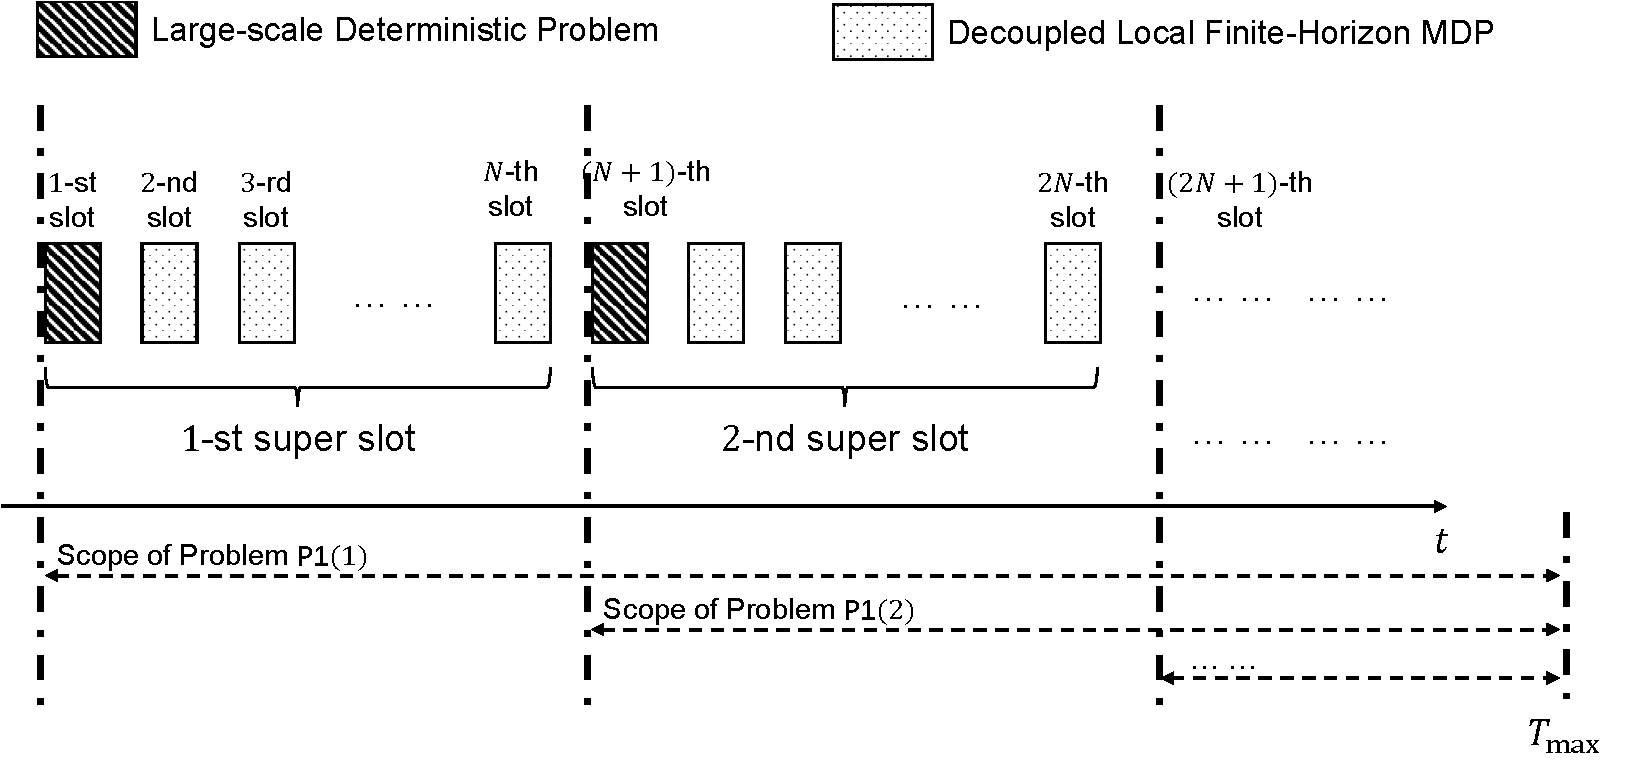
\includegraphics[width=0.90\textwidth]{optimizer-framework.pdf}
    \caption{The illustration of the {\fwName} optimizer framework.}
    \label{fig:optimizer_framework}
\end{figure*}

\section{{\fwName} Simulator for Transition Probability Training}
\label{sec:framework}

The waypoint transition probabilities $\Pr\bracket{\vec{d}_{m,t+1}|\vec{d}_{m,t}}$ ($\forall m\in\carSet$) in equation \eqref{eqn:trans_prob} depend on routes, road topology, microscopic traffic behavior, etc., which are usually difficult to measure in advance.
A mismatching of the trajectories' statistics would lead to a biased estimation of the value function defined in equation \eqref{eqn:p1_val}, and degrade the performance of the optimized scheduling policy. To our best knowledge, there is currently no analytical model for the vehicles' trajectory prediction.
Therefore, we develop the {\fwName} simulator to simulate the trajectories of {\IAVs} for arbitrary traffic scenario, so that the waypoint transition probabilities $\Pr\bracket{\vec{d}_{m,t+1}|\vec{d}_{m,t}}$ can be trained in an offline manner.

The {\fwName} simulator integrates two well-known autonomous driving simulators, namely SUMO \cite{SUMO} and CARLA \cite{CARLA}.
CARLA is the open-source simulator based on Unreal Engine \cite{unrealengine}, which provides customized road topology and vehicle types following the OpenDRIVE specification \cite{OpenDRIVE}.
On the other hand, SUMO provides the traffic management of vehicles with well-defined microscopic traffic flow model.
Based on them, the procedure to train the transition probabilities is given as follows.

\textbf{Road Topology and Traffic Initialization.} In order to simulate the random traffic on the particular scenario, we use CARLA to generate the target road map and leverage the program \emph{ActivityGen} provided by SUMO to generate random traffic demands according to the road map. The traffic demands can be customized by adjusting the following statistics: population distribution, working hours, car-holding rate, vehicular statistics and etc.
The study \cite{sumo-accuracy-mdpi} shows that the traffic flow generated by SUMO could match the traffic conditions of the real world on usual weekdays.

\textbf{Trajectory Dataset Generation.} Based on the above road map and traffic demands, the trajectories of all vehicles can be generated and recorded.
Let $\mathcal{X}_{m} $ be the set of vehicles running on the route of the $m$-th {\IAV} in all the simulation trials, and $$ \vec{x}^{(i)}_{m} = \Paren{ \vec{d}^{(i)}_{m,1}, \vec{d}^{(i)}_{m,2}, \dots }$$ be the trajectory of the $ i $-th vehicle in $\mathcal{X}_{m}$, where $\vec{d}^{(i)}_{m,t} \in \tjSet_{m}$ is the position in the $ t $-th time slot.

\textbf{Waypoint Transition Matrix Training.} Based on the trajectory dataset $ \{\vec{x}^{(i)}_{m} | \forall i,m\} $, the transition matrices for all {\IAVs} waypoint $\{\TransD_{m}| \forall m\}$ defined in equation \eqref{eqn:trans_mat} can be obtained as follows. 
\begin{align*}
    \Paren{\TransD_{m}}_{j,k} = 
        \frac{
            \sum_{t,i} \indicator\bracket{ \vec{d}^{(i)}_{t+1}=\vec{w}_{m,k}, \vec{d}^{(i)}_{t}=\vec{w}_{m,j} }
        }{
            \sum_{t,i}\sum_{l} \indicator \bracket{ \vec{d}^{(i)}_{t+1}=\vec{w}_{m,l}, \vec{d}^{(i)}_{t}=\vec{w}_{m,j} }
        }, \forall j,k.
\end{align*}
As a remark note that the trajectory dataset generation and waypoint transition matrix training are conducted in an offline manner before the uplink transmission, the {\fwName} simulator would have sufficient time to ensure a large number of trajectory samples. 

\begin{figure*}[t]
    \begin{eqnarray}
            \sum_{\tau=kN+1}^{T} g_{\tau}\Paren{
                \mathbb{E}_{\Stat_{\tau}} \Bracket{ \Stat_{\tau} | \Stat_{kN+1} }, \vec{A}_{\tau}
            } 
            &\approx&
            T + \omega \sum_{\tau=kN+1}^{T} \sum_{m\in\carSet} \gamma_{m,\tau}
            2^\frac{r_{m,\tau}}{\gamma_{m,\tau}T_s B_0} 
            \times \xi_{m,\tau} \mathbb{E}_{\Stat_{\tau}} \Bracket{ l_{m,\tau}^{\epsilon}~|~\Stat_{kN+1} } \nonumber\\
            &\define&    F_k\Paren{ T, \mat{R}^{(k,T)}, \mat{\Gamma}^{(k,T)} }
            \label{eqn:fk}
    \end{eqnarray}
    \hrulefill
\end{figure*}

\section{\revise{Decentralized Scheduling Framework of {\fwName} Optimizer}}
\label{sec:new_framework}

The joint policy optimization for the {\IAVs} in problem {\bf P1} suffers from the {\it curse of dimensionality} \cite{mdp-huang,mdp-lv}.
This is because the transmission time and throughput allocation of each {\IAV} in each time slot depend on the global system state (aggregation of the states of all {\IAVs}), whose support grows exponentially with respect to the {\IAV} number. It can be observed that if the transmission time allocation of all {\IAVs} $\{\gamma_{m,t}|\forall m,t\}$ is predetermined, the throughput allocation of each {\IAV} in all the time slots can be optimized without the consideration of other {\IAVs}' states. However, fixing the the transmission time allocation of all {\IAVs} before the model uploading would degrade the performance, as they could not be adjusted according to the real-time positions and remaining information bits of all {\IAVs}.

In order to reduce the computational complexity and meanwhile maintain the performance gain of dynamic programming, a dynamic decoupling method is proposed for the {\fwName} optimizer in this section. The framework is illustrated in Fig. \ref{fig:optimizer_framework}, where every $N$ time slots is organized as a {\it super slot} and the online optimization consists of the following two time scales.
\begin{itemize}
    \item Super-slot scale: the transmission time allocation of all {\IAVs} for the remaining time slots is periodically optimized at the beginning of each super slot. Such optimization will be approximated as a deterministic optimization problem based on the global system state at the beginning of each super slot.
    \item Slot scale: based on transmission time allocation, the optimization of throughput allocation policy of each {\IAV} for all the remaining time slots can be decoupled as a local finite-horizon MDP with tractable state space. The approximate expressions of local value functions will be derived, such that each {\IAV} can evaluate them and determine the throughput allocation in each slot without the effort of offline value iteration.
\end{itemize}

\subsection{Super-Slot Scale Optimization}
Without loss of generality, we consider the scheduling since the $k$-th super slot (from the $(kN+1)$-th time slot), where $k=1,2,\dots$. The policy optimization of problem {\bf P1} for all the remaining time slots given the global system state $\Stat_{kN+1}$ reduces to the following sub-problem:
\begin{align}
    \textbf{P1$(k)$:}
    \nonumber\\ 
    &\min_{ \Policy_{kN+1}, \dots, \Policy_\T }
        \sum_{\tau=kN+1}^{\T}  \mathbb{E}_{\Stat_{\tau}} \Bracket{
            g_{\tau}\paren{ \Stat_{\tau}, \vec{A}_{\tau} } | \Stat_{kN+1}
        } \nonumber
    \\ \nonumber
    \text{s.t.~~} &\text{\eqref{eqn:p1_cons_second}, \eqref{eqn:p1_cons_last}, \eqref{eqn:p1_cons_first}},
    \\
    & \sum_{ \tau=\max\paren{kN+1,T_{\text{comp},m}} }^{ \T } r_{m,\tau} \geq {u}_{m,kN+1}, \forall m\in\carSet,
    \label{eqn:p1p_cons_last}
\end{align}
where the last constraint \eqref{eqn:p1p_cons_last} is to ensure all the data in the uplink queues of {\IAVs} should be delivered.


In the optimization of super-slot scale, the average trajectories are used as the representatives to optimize the time slot allocation, such that the dynamic programming of problem \textbf{P1$(k)$} can be simplified to a deterministic optimization problem.
Note that
\begin{align}
    \sum_{\tau=kN+1}^{\T} g_{\tau}\Paren{
        \mathbb{E}_{\Stat_{\tau}}\Bracket{ \Stat_{\tau} | \Stat_{kN+1} }, \vec{A}_{\tau}
    }
    \label{eqn:cost_approx}
\end{align}
represents the system cost with the average trajectory
\begin{align}
    \Paren{
        \mathbb{E}\Bracket{ \vec{d}_{m,kN+1} | \vec{d}_{m,kN+1} },
        \dots,
        \mathbb{E}\Bracket{ \vec{d}_{m,T} | \vec{d}_{m,kN+1} }
    }
\end{align}
of the $m$-th {\IAV} ($\forall m\in\carSet$) since the $k$-th super slot. Approximating the objective by \eqref{eqn:cost_approx}, the policy optimization in problem \textbf{P1$(k)$} can be simplified into the following deterministic optimization of transmission time and throughput for the above average trajectories.
    \begin{align}
        \textbf{P2$(k)$:~} &
        ~~~\Paren{T^{(k,*)}, \mat{R}^{(k,*)}, \mat{\Gamma}^{(k,*)} }\nonumber \\
        & = \arg\min_{ T, \mat{R}^{(k,T)}, \mat{\Gamma}^{(k,T)} } F_k\Paren{ T, \mat{R}^{(k,T)}, \mat{\Gamma}^{(k,T)} }\nonumber
            \\
        &\text{s.t.~} \text{ \eqref{eqn:p1_cons_second}, \eqref{eqn:p1_cons_last}, \eqref{eqn:p1_cons_first},}
        \nonumber\\
    & \sum_{ \tau=kN+1 }^{ T } r_{m,\tau} \geq {u}_{m,kN+1} \forall m\in\carSet, \label{eqn:constraint_T}
    \end{align}
where
$$
\mat{\Gamma}^{(k,T)} \define [ \gamma^{(k)}_{m,kN+\tau} ]_{1 \leq m \leq M, 1 \leq \tau \leq T-kN} \in \domR^{M \times (T-kN)}
$$
and
$$\mat{R}^{(k,T)} \define [ r^{(k)}_{m,kN+\tau}]_{1 \leq m \leq M, 1 \leq \tau \leq T-kN} \in \domR^{M \times (T-kN)}$$
are the aggregation matrices of time and throughput allocations of all the remaining time slots for the above average trajectories, respectively. $T$ denotes the number of slots in the scheduling period. $F_k(\cdot)$ is defined in \eqref{eqn:fk}, where the high-SNR approximation on power consumption
\begin{align}
    p_{m,t} \approx \xi_{m,t} l_{m,t}^{\epsilon} 2^{\frac{ r_{m,t} }{ \gamma_{m,t} T_{s} B_0 }},
\end{align}
with $\xi_{m,t} = \frac{N_0}{\kappa \sigma^\epsilon} 2^{-\mathbb{E}_{h_{m,t}}\bracket{\log_2{|h_{m,t}|^2}}}$ is used.


The  algorithm for the super-slot scale optimization in problem \textbf{P2$(k)$} is discussed in Section \ref{sec:kernel-policy}.
Its solution is denoted as
$$\mat{\Gamma}^{(k,*)}=[\gamma^{(k,*)}_{m,\tau+kN}]_{1 \leq m \leq M, 1 \leq \tau \leq T^{(k,*)}-kN}$$
and
$$\mat{R}^{(k,*)}=[r^{(k,*)}_{m,\tau+kN}]_{1 \leq m \leq M, 1 \leq \tau \leq T^{(k,*)}-kN},$$
where $$\Brace{ \vecG{\gamma}^{(k,*)}_{m,\tau} | \forall m\in\carSet, \tau=kN+1,\dots,(k+1)N }$$ are adopted as the time allocation of the $k$-th super slot.


\noindent{\bf Remark:} {\it In high SNR region, with the optimized time $\mat{\Gamma}^{(k,*)}$ and throughput $\mat{R}^{(k,*)}$ allocations, the system cost with the average trajectory equals the average system cost with random trajectories. Thus,
\begin{align*}
F_k &\Paren{ T^{(k,*)}, \mat{R}^{(k,*)}, \mat{\Gamma}^{(k,*)}} =
\nonumber\\
&\sum_{\tau=kN+1}^{T^{(k,*)}} \mathbb{E}_{\Stat_{\tau}} \Bracket{
            g_{\tau}\paren{ \Stat_{\tau}, \gamma^{(k,*)}_{m,\tau}, r^{(k,*)}_{m,\tau}} | \Stat_{kN+1}
        }.
\end{align*}
This will be exploited to derive a non-trivial performance bound of the proposed algorithm.}

\subsection{Decoupled Optimization in Slot Scale}
In the slot scale, with the optimized time allocation $\mat{\Gamma}^{(k,*)}$ and optimized length of scheduling period $T^{(k,*)}$ in the previous part, the throughput allocation policies of {\IAVs} can be decoupled. We first define the following local throughput allocation policies for the $m$-th {\IAV} ($\forall m\in\carSet$):
\begin{align}
    \Policy^{R}_{m,t}( \Stat_{m,t} ) = r_{m,t},~t=kN+1,\dots,T^{(k,*)}.
\end{align}
Moreover, the local cost function of the $m$-th {\IAV} in the $t$-th time slot can be decoupled from (\ref{eqn:func_g})  as
\begin{align}
    g_{m,t}\Paren{ \Stat_{m,t}, \Policy^{R}_{m,t}(\Stat_{m,t}) } = \gamma^{(k,*)}_{m,t} p_{m,t}.
\end{align}
Then the optimization of the local throughput allocation policies for the $m$-th {\IAV} can be written as follows:
\begin{align}
    \textbf{P3$(k,m)$:~}
    &\min_{ \set{\Policy^{R}_{m,\tau} | \tau=kN+1,\dots,T^{(k,*)} } }
        \nonumber\\
        &\sum_{\tau=kN+1}^{T^{(k,*)}}
        \mathbb{E}_{\Stat_{m,\tau}} \Bracket{
            g_{m,\tau}\Paren{ \Stat_{m,\tau}, \Policy^{R}_{m,\tau}( \Stat_{m,\tau} ) }\nonumber
        }
    \\\nonumber
    &\text{s.t.~} \text{ \eqref{eqn:p1_cons_second}, \eqref{eqn:p1_cons_last}, \eqref{eqn:p1_cons_first}, } \nonumber\\
    & ~~~ \sum_{ \tau=\max\paren{kN+1,T_{\text{comp},m}} }^{ T^{(k,*)}} r_{m,\tau} \geq {u}_{m,kN+1}.
\end{align}

Note that the above problem \textbf{P3$(k,m)$} is a finite-horizon MDP based on the local system state, it can be optimized locally at the $m$-th {\IAV}. The analytical expressions to approximate its local value functions will be proposed. Hence, at the beginning of each slot in the $k$-th super slot, the $m$-th {\IAV} first evaluates the next slot's local value function, and then determines the throughput allocation action of the current slot  according to the current local system state. The solution will be discussed in Section \ref{sec:local-policy}.
